%%%%%%%%%%%%%%%%%%%%%%%%%%%%%%%%%%%%%%%%%%%%%%%%%%%%%%%%%%%%%%%%%%%%%%%%%%%%%%%%
% Лабораторная работа 4 : Определение модуля сдвига G.
% Выполнили             : Баталов Семен, Хайретдинова Диана, 2021.
%%%%%%%%%%%%%%%%%%%%%%%%%%%%%%%%%%%%%%%%%%%%%%%%%%%%%%%%%%%%%%%%%%%%%%%%%%%%%%%%

\documentclass[12pt, a4paper]{article}
\usepackage[left=2cm, right=2cm, top=2.5cm, bottom=2.5cm, nohead]{geometry}
\usepackage{graphicx}
\usepackage[utf8]{inputenc}
\usepackage[english, russian]{babel}
\usepackage{indentfirst}
\usepackage{amsmath}
\usepackage{longtable}
\usepackage{multirow}
\usepackage{array}
\usepackage{rotating}
\usepackage{subcaption}
\graphicspath{{./Figures/}}

\begin{document}
    
    \newcolumntype{M}[1]{>{\centering\arraybackslash}m{#1}}
    \renewcommand{\arraystretch}{1.4}
    
    \begin{center}
        \large{Санкт-Петербургский Государственный Университет} \\
        \large{Saint-Petersburg State University}\\
        \hfill \break
        \hfill \break
        \hfill \break
        \hfill \break
        \hfill \break
        \hfill \break
        \large{ЛАБОРАТОРИЯ ПРОЧНОСТИ МАТЕРИАЛОВ} \\
        \hfill \break
        \hfill \break
        \hfill \break
        \large{\textbf{ОТЧЕТ}} \\
        \large{\textbf{По лабораторной работе 4}} \\
        \large{<<Определение модуля сдвига G>>} \\
        \hfill \break
        \hfill \break
        \hfill \break
        \large{По дисциплине} \\
        \large{<<Лабораторный практикум, лабораторная работа>>} \\
    \end{center}
    
    \hfill \break
    \hfill \break
    \hfill \break
    \hfill \break
    \hfill \break
    \hfill \break
    
    \begin{flushright} 
        \large{Выполнили:} \\
        \hfill \break
        \large{Баталов С. А.} \\
        \large{Хайретдинова Д. Д.} \\
    \end{flushright}
    
    \hfill \break
    \hfill \break
    \hfill \break
    \hfill \break
    \hfill \break
    
    \begin{center} 
        \large{Санкт-Петербург} \\
        \large{2021} \\
    \end{center}
    
    \thispagestyle{empty}
    \newpage
    \sloppy
    
    \section{Экспериментальная установка}
    
    Установка для определения модуля сдвига $G$ (рис.~\ref{im1}) состоит из стойки \textit{1}, на верхнем конце которой закреплена горизонтальная планка с зажимом для испытуемого стержня \textit{2} радиусом $r$. На нижнем конце стержня укреплен диск \textit{3} с проточкой по окружности. Две подвески с грузами \textit{4} предназначены для создания крутящего момента $M_\text{кр}$. При нагружении нижний конец стержня поворачивается на угол $\varphi$. Значение его можно определить при помощи светового зайчика от зеркала, укрепленного под диском \textit{3}. Схема установки зрительной трубы, зеркала и шкалы показана на рис.~\ref{im1}.
    
    \begin{figure}[h]
        \centering
        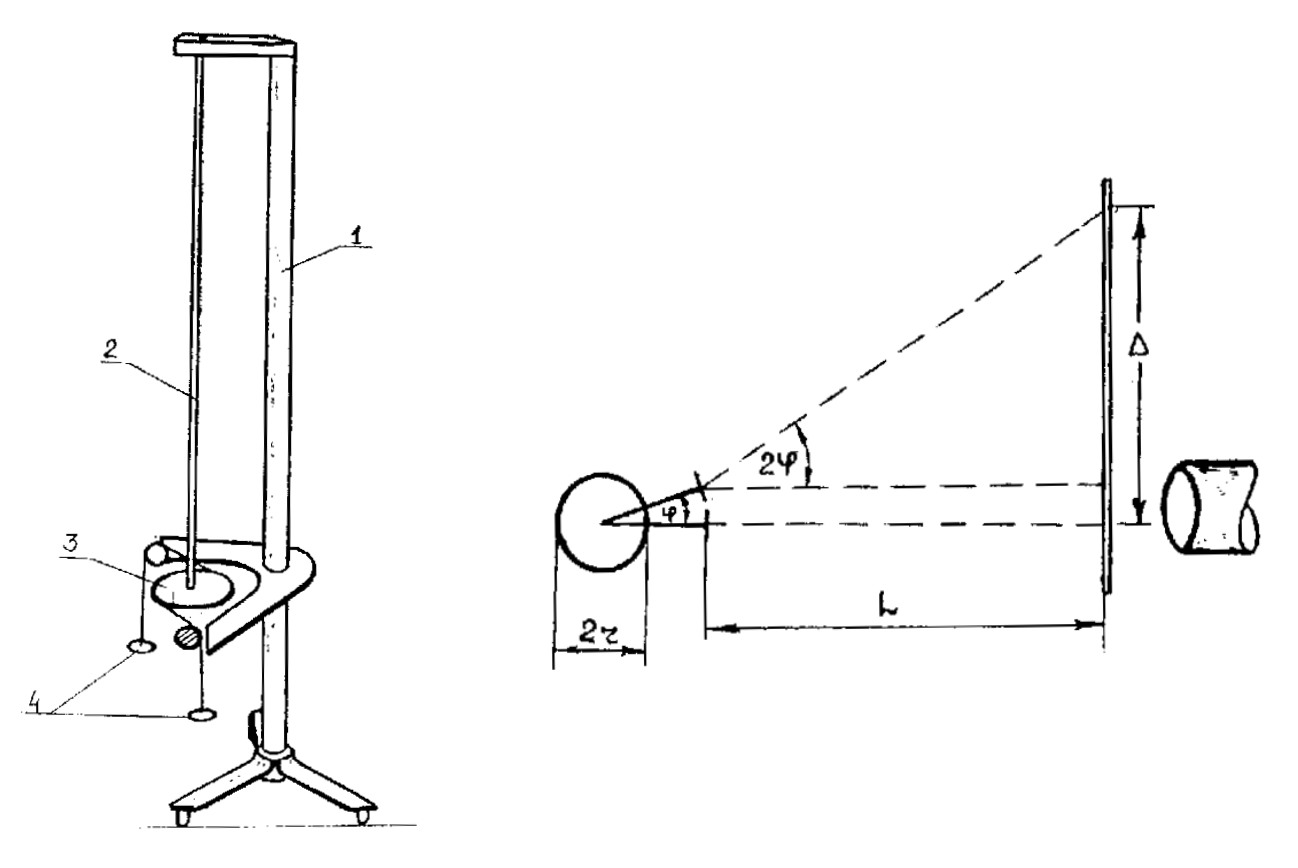
\includegraphics[width = 16cm]{image_1.png}
        \caption{Схема лабораторной установки.}
        \label{im1}
    \end{figure}
    
    \newpage
    
    \section{Теоретические исследования}
    
    \begin{figure}[h]
        \centering
        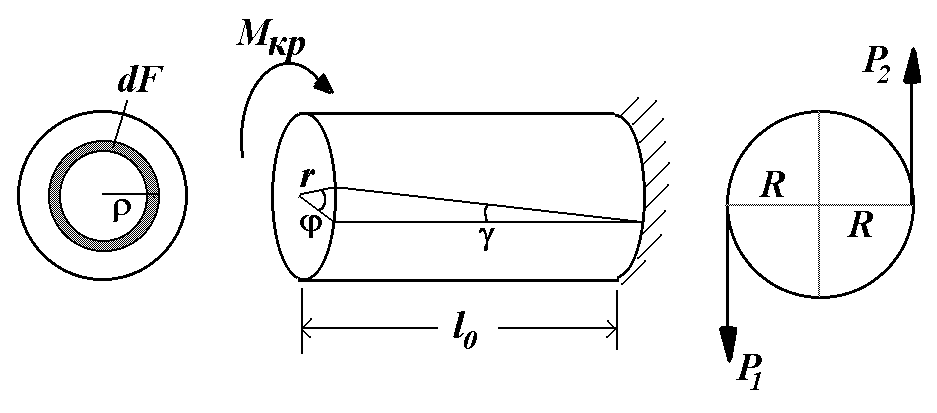
\includegraphics[width = 10cm]{image_2.png}
        \caption{Определение модуля сдвига.}
        \label{im2}
    \end{figure}
    
    Модуль $G$ можно расчитать для состояния чистого сдвига при кручении стержня. Требуется определить по начальным данным угол поворота, для малых величин значение этого угла $\varphi$ (рис.~\ref{im2}) определяют по следующей формуле:
    \begin{equation}
        \varphi = \frac{\Delta}{2L},
        \label{eq1}
    \end{equation}
    где $\Delta$~--~смещение зайчика на шкале, $L$~--~расстояние от шкалы до зеркала. Величину $L$ выбирают в пределах  от 100~см до 150~см.
    
    Значение модуля сдвига $G$ можно получить из закона Гука:
    \begin{equation}
        G = \frac{\tau}{\gamma},
        \label{eq2}
    \end{equation}
    где $\tau$~--~касательное напряжение, $\gamma$~--~деформация сдвига.
    
    Из решения задачи о кручении круглого стержня известно, что касательное напряжение на поверхности стержня равняется:
    \begin{equation}
        \tau = \frac{M_\text{кр}r}{J_{p}},
        \label{eq3}
    \end{equation}
    где $r$~--~радиус стержня, $M_\text{кр} = R(P_{1} + P_{2})$~--~крутящий момент (рис.~\ref{im2}), $J_{p} = \int_{F} \rho^{2} dF$~--~полярный момент инерции стержня, вычисляем по формуле:
    \begin{equation}
        J_{p} = \frac{\pi}{2} r^{4}.
        \label{eq4}
    \end{equation}
    
    Деформация сдвига связана с углом поворота нижнего сечения $\varphi$ соотношением:
    \begin{equation}
        \gamma l_{0} = r\varphi,
        \label{eq5}
    \end{equation}
    где $l_{0}$~--~длина стержня (на нашей установке $l_{0} = 129~\text{см}$).
    
    Из соотношений (\ref{eq1})~--~(\ref{eq5}) имеем окончательное выражение для модуля сдвига:
    \begin{equation}
        G = \frac{M_{\text{кр}}l_{0}}{J_{p}\varphi} = \frac{8 P R l_{0} L}{\pi \Delta r^{4}}.
        \label{eq6}
    \end{equation}
    
    \newpage
    
    \section{Эксперимент}
    
    В данной работе при плоском напряженном состоянии проводится определение модуля сдвига $G$. Важно отметить, что все вычисления и построения производились с помощью пакета Matlab, с исходным кодом программы можно ознакомиться отдельно. Данные установки представлены в таблице~\ref{tb1}.
    
    \begin{table}[h]
        \centering
        \begin{tabular}{| M{3cm} | M{3cm} | M{3cm} |}
            \hline
            Величина & Значение & Размерность \\
            \hline
            $R$ & 55.2 & \multirow{2}{*}{мм} \\
            $r$ & 3.05 & \\
            \hline
            $L$ & 107 & \multirow{2}{*}{см} \\
            $l_{0}$ & 129 & \\
            \hline
        \end{tabular}
        \caption{\centering Начальные данные.}
        \label{tb1}
    \end{table}
    
    Результаты измерений представлены в таблице~\ref{tb2}. Замер производился дважды, причем каждый раз производилось плавное нагружение и плавное разгружение.
    
    \begin{table}[h]
        \centering
        \begin{tabular}{| M{1.5cm} | M{2cm} | M{3cm} |M{3cm}|}
            \hline
            \multirow{3}{*}{№} & \multirow{2}{*}{P} & \multicolumn{2}{c|}{$\Delta$} \\
            \cline{3-4}
            & & Замер №1 & Замер №2 \\
            \cline{2-4}
            & кг & \multicolumn{2}{c|}{cм} \\
            \hline
            1  & 0    & 12.2 & 12.3 \\
            2  & 0.05 & 13.6 & 13.6 \\
            3  & 0.1  & 15   & 15   \\
            4  & 0.15 & 16.3 & 16.4 \\
            5  & 0.2  & 17.7 & 17.9 \\
            6  & 0.25 & 19.1 & 19.2 \\
            7  & 0.3  & 20.6 & 20.6 \\
            8  & 0.35 & 21.9 & 22   \\
            9  & 0.3  & 20.9 & 20.8 \\
            10 & 0.25 & 19.4 & 19.4 \\
            11 & 0.2  & 18.1 & 18   \\
            12 & 0.15 & 16.6 & 16.6 \\
            13 & 0.1  & 15.2 & 15.1 \\
            14 & 0.05 & 13.7 & 13.7 \\
            15 & 0    & 12.3 & 12.3 \\
            \hline
        \end{tabular}
        \caption{\centering Результаты измерений.}
        \label{tb2}
    \end{table}
    
    \newpage
    
    Далее представлены графики в координатах $M_{\text{кр}}$~--~$\varphi$ и $\tau$~--~$\gamma$. На них изображены кривые соответствующие как нагружению стержня, так и его разгружению.
    
    \begin{figure}[h]
        \centering
        \begin{subfigure}{\textwidth}
            \centering
            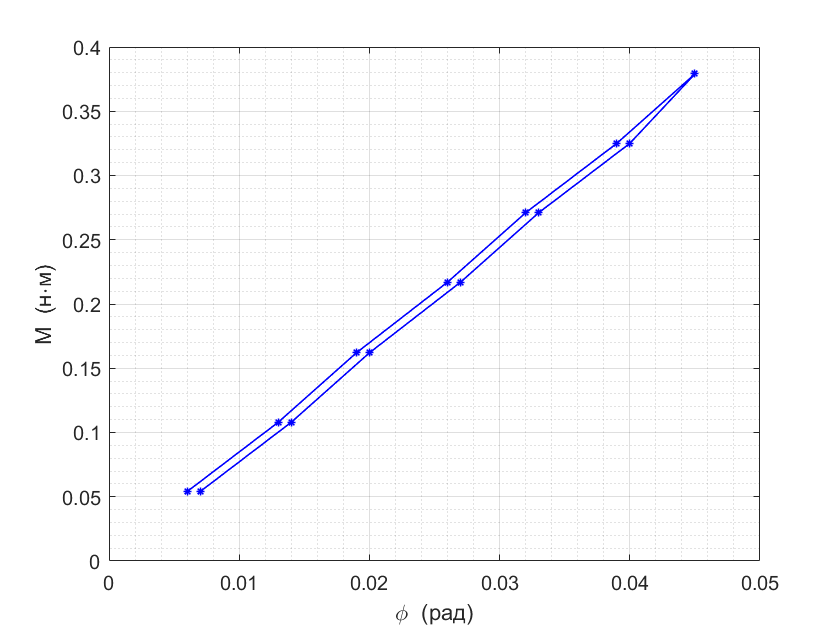
\includegraphics[width = 12cm]{figure_1.png}
        \end{subfigure}
        \begin{subfigure}{\textwidth}
            \centering
            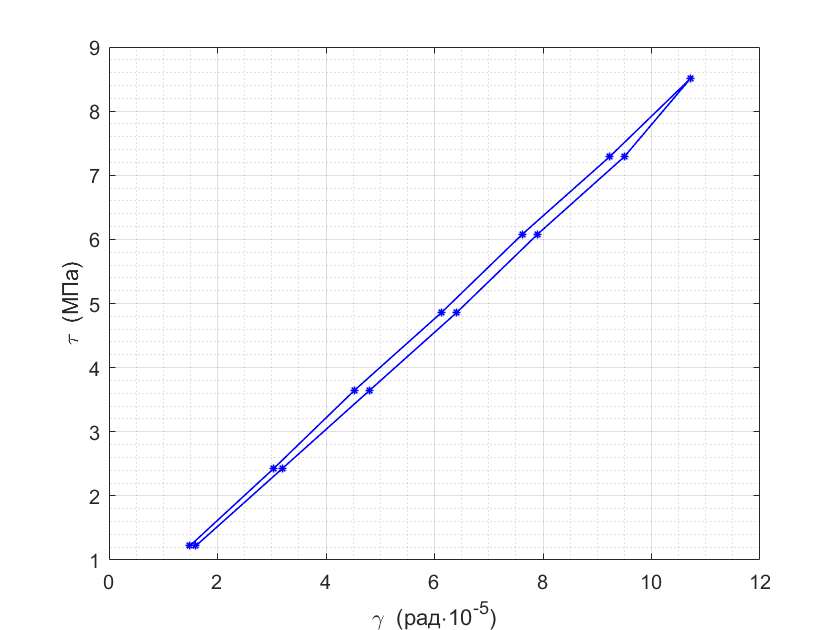
\includegraphics[width = 12cm]{figure_2.png}
        \end{subfigure}
        \caption{Графики в координатах $M_{\text{кр}}$~--~$\varphi$ и $\tau$~--~$\gamma$.}
        \label{fig1}
    \end{figure}
    
    Видно, что зависимости являются линейными,при этом прямая нагружения сохраняет параллельность прямой разгружения в обоих случаях. При построении графиков использовались не все значения выборки. Были отброшены крайние точки, в которых отсутствовал нагружающий момент.
    
    \begin{sidewaystable}
        \centering
        \begin{tabular}[p]{| M{1cm} | M{2cm} | M{2cm} | M{2cm} | M{2cm} | M{2cm} | M{2cm} | M{2cm} | M{2cm} | M{2cm} |}
            \hline
            \multirow{2}{*}{№} & $P$ & $\Delta$ & $\varphi$ & $M_{\text{кр}}$ & $\tau$ & $\gamma$ & $G$ & $\Delta G$ & $\varepsilon$ \\
            \cline{2-10}
            & Н & м & рад & Н $\cdot$ м & МПа & $\cdot 10^{-5} \, \text{рад}$ & \multicolumn{2}{c|}{ГПа} & \% \\
            \hline
            1 & 0.491 & 0.014 & 0.006 & 0.054 & 1.22 & 1.49 & 81.5 & 24.5 & 30 \\
            2 & 0.981 & 0.027 & 0.013 & 0.108 & 2.43 & 3.04 & 80.0 & 14.9 & 19 \\
            3 & 1.472 & 0.041 & 0.019 & 0.162 & 3.65 & 4.53 & 80.5 & 10.6 & 13 \\
            4 & 1.962 & 0.055 & 0.026 & 0.217 & 4.86 & 6.13 & 79.3 & 11.6 & 15 \\
            5 & 2.453 & 0.069 & 0.032 & 0.271 & 6.08 & 7.62 & 79.7 & 10.5 & 13 \\
            6 & 2.943 & 0.084 & 0.039 & 0.325 & 7.29 & 9.23 & 79.0 & 10.9 & 14 \\
            7 & 3.434 & 0.097 & 0.045 & 0.379 & 8.51 & 10.72 & 79.4 & 10.4 & 13 \\
            8 & 2.943 & 0.086 & 0.040 & 0.325 & 7.29 & 9.50 & 76.7 & 11.8 & 15 \\
            9 & 2.453 & 0.071 & 0.033 & 0.271 & 6.08 & 7.90 & 76.9 & 10.8 & 14 \\
            10 & 1.962 & 0.058 & 0.027 & 0.217 & 4.86 & 6.41 & 75.8 & 13.3 & 18 \\
            11 & 1.472 & 0.044 & 0.020 & 0.162 & 3.65 & 4.81 & 75.8 & 11.8 & 16 \\
            12 & 0.981 & 0.029 & 0.014 & 0.108 & 2.43 & 3.20 & 75.8 & 20.4 & 27 \\
            13 & 0.491 & 0.014 & 0.007 & 0.054 & 1.22 & 1.60 & 75.8 & 21.5 & 28 \\
            \hline
        \end{tabular}
        \label{tb3}
        \caption{\centering Результаты измерений и расчеты.}
    \end{sidewaystable}
    
    \newpage
    
    \section{Выводы}
    
    В данной работе был экспериментально найден модуль сдвига стали, был проведен эксперимент со стержнем из этого металла, в процессе которого последний был подвержен действию крутящего момента, что в свою очередь, породило в стержне напряженное состояние. Далее были измерены параметры этого напряженного состояния с помощью оптической регистрирующей системы, результаты были обработаны инструментами пакета Matlab. В ходе работы вычислялись погрешности систематические, статистические и погрешности косвенных измерений.
    
    В результате проделанной работы был получен модуль сдвига $G$ для стали, его значение в среднем по всей выборке составило:
    \begin{equation}
        G = 80 \pm 13 \, \text{ГПа},
        \label{eq7}
    \end{equation}
    данный результат хорошо согласуется с действительным значения модуля сдвига для этого металла. В заключении, поставленная задача была решена, основные цели работы были достигнуты, и полученный модуль сдвига хорошо согласуется с действительным значением.
    
\end{document}